%!TEX root = ../TFM.tex



\chapter{Gamificar las Matemáticas}

%Lo que debes reflfejar en este capítulo es cómo lo has hecho, cual es tu objetivo, como organizas el aula, como lo evaluas y qué resultados obtienes.

%Una vez explicitados los fundamentos sobre los que basamos nuestra propuesta metodológica, procedemos a su descripción.

%\section{Objetivos}

El principal objetivo es ofrecer una propuesta de trabajo que suponga una innovación y una mejora en el actual sistema educativo.
%
Para ello, ofrecemos una concreción de la metodología estudiada con la que desarrollar una Unidad Didáctica.
% 
Por otro lado, se espera que esta propuesta suponga para los alumnos un proceso de enseñanza-aprendizaje en el que puedan adquirir las competencias y aprendizajes necesarios de una manera más profunda, duradera y entretenida.

%Para ello, se desarrollará la propuesta y después se ofrecerá un marco de investigación\crossref{ (ver \ref{evalGami})} para evaluar si esta propuesta metodológica supone realmente una innovación y una mejora.

\section{Diseño de la gamificación}

Se ha tratado, en términos generales, la propuesta para diseñar una gamificación de \cite{kapp2013gamification}. 
%
Se va a utilizar esa propuesta para guiar el proceso de diseño de la gamificación. 
%
Para ello, se irán recorriendo las etapas propuestas.

El primer paso consiste en estudiar el problema que se quiere resolver. 
%
Éste ha sido tratado con amplitud anteriormente\crossref{(ver sección \ref{chap:intro})}, estudiando los comportamientos existentes. 
%
Por otro lado, el comportamiento deseado sería que los estudiantes estuvieran más motivados y comprometidos con la asignatura, dispuestos a trabajar activamente en clase y autónomamente en casa.

Además, el objetivo competencial está definido por el \bocm y se detallará más adelante\crossref{(ver \ref{tbl:Matrizdetodo})}.

El último aspecto de las preguntas base es la valoración de los aspectos que puedan darnos retroalimentación sobre el proceso.
%
La manera en la que se va a conseguir eso es mediante el diseño de un itinerario de logros y puntos que los alumnos van recorriendo.
%
De esta manera se puede anticipar fácilmente si hay algún alumno rezagado simplemente observando los logros adquiridos y los puntos.
%
No obstante, en cada sesión y tarea se especificará un mínimo a alcanzar por parte de los alumnos.

En el segundo paso se trabajan las preguntas prácticas.
%
El público objetivo de la gamificación son alumnos de secundaria del sistema educativo español. 
%
Debido a que esta gamificación no se plantea para ser aplicada en un centro en concreto, no se pueden determinar con exactitud los conocimientos previos y habilidades ni los tipos de jugadores concretos a los que esta propuesta se dirige.

No obstante, en este trabajo se han tratado los tipos de jugadores\crossref{ (ver \ref{sec:taxonomy})} para que el docente, en el momento de implantación de esta gamificación pueda definir los tipos de jugadores concretos a quienes se dirige la gamificación.
%
Por otro lado, la definición logística y técnica de la gamificación se encuentra especificado a lo largo de la descripción de la unidad didáctica\crossref{ (ver sección \ref{sec:UD})}. 

Asimismo, el sistema de valoración también está incluido en la unidad didáctica, anticipando durante el diseño los posibles fallos del sistema para conseguir una evaluación lo más justa posible.

El último paso de la propuesta de \cite{kapp2013gamification} sería la puesta en marcha del sistema. 
%
Desafortunadamente, esta gamificación no ha podido ser llevada al aula todavía.

\subsection{Marco legal de aplicación}

La \lomce establece que: \comillas{Necesitamos propiciar las condiciones que permitan el oportuno cambio metodológico, de forma que el alumnado sea un elemento activo en el proceso de aprendizaje.} 
%
En este sentido, nuestra propuesta metodológica se apoya en las indicaciones establecidas por la \lomce para el ejercicio de la labor docente.

La \lomce establece condiciones generales que son concretadas por el \boe, estableciendo los contenidos que se deben tratar en cada curso.
%
Después, corresponde a cada Administración la elaboración del currículo básico para su comunidad autónoma.
%
En este caso, recurrimos al \bocm.


\subsection{Elección del curso para Gamificar}

El curso elegido para desarrollar la propuesta es Matemáticas Orientadas a las Ciencias Académicas de 3º de ESO por ser 3º de ESO el curso en el que se constata que se ha producido un aumento del rechazo hacia las Matemáticas\crossref{ (ver sección \ref{sec:estudioNacional})}.
%
Además, es también el curso en el que la percepción de la asignatura como divertida es menor: 40,46\% en 3º de ESO frente a 54,46\% en Bachillerato y 68,51\% en 1º de ESO \citep{ActitudesHaciaMates}.

Dentro del curso se ha escogido desarrollar una unidad didáctica sobre polinomios porque es el primer curso en el que se tratan los polinomios y su mal aprendizaje puede lastrar al alumno el resto de su trayectoria en el sistema educativo, incluso hasta los primeros cursos universitarios.
%
La factorización de polinomios, por ejemplo, es un recurso importante en la diagonalización de matrices, contenido fundamental en Álgebra de cualquier grado en Ingeniería o Administración y Dirección de Empresas.


Si en este curso se consigue un aprendizaje consolidado y duradero, los estudiantes podrán desempeñar y aprovechar mejor los cursos venideros.


\section{Unidad didáctica gamificada}

\label{sec:UD}
%
Esta unidad didáctica pertenece a la asignatura Matemáticas Orientadas a las Ciencias Académicas de 3º ESO. 
%
Los contenidos de la asignatura, definidos en el \boe y matizados por el \bocm, se dividen en 5 bloques:
1) Procesos métodos y actitudes en las matemáticas. 
2) Números y álgebra: Números racionales, números decimales, polinomios, sucesiones, ecuaciones y sistemas.
3) Geometría: geometría plana, geometría del espacio, globo terráqueo, uso de herramientas tecnológicas.
4) Funciones.
5) Estadística y probabilidad.

Esta unidad didáctica pertenece al bloque de Números y Álgebra para tratar el punto 6 de los contenidos del bloque 2 según el \bocm: \comillas{Polinomios. Expresiones algebraicas.}
%
Este punto incluye:
%
\comillas{Transformación de expresiones algebraicas, igualdades notables, operaciones elementales con polinomios. 
%
Ecuaciones de primer y segundo grado con una incógnita y resolución por el método algebraico y gráfico de ecuaciones de primer y segundo grado.}
%
Más adelante, en la tabla \ref{tbl:Matrizdetodo} se expondrán más claramente los Contenidos, Criterios de Evaluación y \eaes pertinentes.

Esta unidad didáctica desarrollará todo lo relativo a polinomios y su manejo, excluyendo las ecuaciones y sistemas de ecuaciones que corresponderán a otra unidad didáctica diferente.

\subsection{Conocimientos previos}

Es fundamental que los alumnos recuerden las propiedades de las potencias de exponentes naturales con las que llevan trabajando al menos 2 cursos.
%
Asimismo, sería conveniente que los estudiantes recordaran qué es una expresión algebraica y cómo calcular su valor numérico.
%
No obstante, esto último será repasado en el desarrollo de esta unidad didáctica para corregir posibles desequilibrios entre los niveles de los alumnos.



\subsection{Contenidos y Estándares de Aprendizaje Evaluables}

En la tabla \ref{tbl:Matrizdetodo} se encuentran resumidos los Contenidos, Criterios de Evaluación y  Estándares de Aprendizaje Evaluables de la unidad didáctica desarrollada.

\begin{table}[hbt]
\centering
\caption{Matriz de Contenidos, Criterios de Evaluación y  Estándares de Aprendizaje Evaluables de la unidad didáctica}
\label{tbl:Matrizdetodo}
\begin{tabular}{|p{0.24\linewidth}|p{0.3\linewidth}|p{0.42\linewidth}|}
\hline
 \multicolumn{1}{|c|}{Contenidos} & \multicolumn{1}{|c|}{Criterios de Evaluación} & \multicolumn{1}{c|}{\eaes}
\\\hline

\mylabel{C261}{Cont. 2.6.1} Transformación de expresiones algebraicas. 
&
\multirow{3}{\linewidth}{\mylabel{CE23}{C.E. 2.3} Utilizar el lenguaje algebraico para expresar una propiedad o relación dada mediante un enunciado, extrayendo la información relevante y transformándola.\vfill}
& 
\mylabel{EAE3.1}{E.A.E. 3.1}: Realiza operaciones con polinomios y los utiliza en ejemplos de la vida cotidiana.
\\\cline{1-1} \cline{3-3} 

\mylabel{C262}{Cont. 2.6.2} Igualdades notables. 
&
& 
\mylabel{EAE3.2}{E.A.E. 3.2}: Conoce y utiliza las identidades notables correspondientes al cuadrado de un binomio y una suma por diferencia, y las aplica en un contexto adecuado. 
\\\cline{1-1} \cline{3-3} 

\mylabel{C263}{Cont. 2.6.3} Operaciones elementales con polinomios. 
&
&
\mylabel{EAE3.3}{E.A.E. 3.3}: Factoriza polinomios de grado 4 con raíces enteras mediante el uso combinado de la regla de Ruffini, identidades notables y extracción del factor común.
\\\hline
\end{tabular}
\end{table}
\FloatBarrier

\subsection{Metodología:}

La metodología principal aplicada en esta unidad didáctica será la gamificación.
%
Ésta se apoyará de otras estrategias metodológicas como la colaboración y el trabajo en grupo para la realización de algunos trabajos concretos, el trabajo autónomo y la exposición en la pizarra o con proyecciones por parte del docente.

Con esta metodología específica se pretende aportar las condiciones necesarias para que el aprendizaje de los alumnos sea significativo, funcional y duradero.
%
También aporta un enfoque lúdico y emocionante al aprendizaje ya que, como es bien sabido, sin emoción no tiene lugar el aprendizaje.
%
Además, esta elección metodológica permite hacer protagonista al alumno durante el proceso logrando que se involucre activamente en el proceso de enseñanza-aprendizaje, como sugiere la \lomce.
%
%Por último es una metodología tremendamente flexible que permite sinergias con otras metodologías como el aprendizaje cooperativo y la clase invertida.


Los elementos de la gamificación utilizados son la narrativa, los logros y medallas, los puntos de reputación, que a su vez sirven para comprar bienes reales en una economía de fichas, los retos (que pueden ser retomados varias veces) y un desafío complicado al final de la Unidad Didáctica a modo de jefe final.
%
En el trabajo en casa también se incorporan la retroalimentación inmediata en la realización de los deberes (mediante una plataforma online) y la posibilidad de tomar decisiones sobre los deberes a realizar.

Otro aspecto de la estrategia metodológica es la utilización de herramientas \gls{TIC}, sobre las que la \lomce establece que \comillas{serán una pieza fundamental para producir el cambio metodológico que lleve
a conseguir el objetivo de mejora de la calidad educativa.}
%
Los ejercicios de trabajo autónomo por parte del estudiante en horario no lectivo serán realizados en una plataforma online (\textit{edmodo}) de tal manera que el estudiante pueda recibir feedback inmediato de su desempeño.

Salvo que se especifique lo contrario, no es relevante el tiempo empleado en la resolución de estos ejercicios sino su resolución satisfactoria o insatisfactoria.
%
Se fomentará la corrección en las respuestas más que la rapidez ofreciendo la posibilidad de retomar el ejercicio hasta 3 veces, para facilitar el aprendizaje a partir de los errores y los fallos.

En algunos momentos se trabajará por grupos.
%
Los grupos serán de 4 personas y se buscarán que estén equilibrados.
%
Se utilizarán las notas de Matemáticas del año pasado para equilibrar la competencia matemática de los distintos grupos y el conocimiento del docente de los alumnos para crear grupos que puedan funcionar de la mejor manera posible: separando mejores amigos, separando enemigos (si así se considera) y separando parejas.
%
\label{grupos}
%
Los grupos se crearán el primer día y siempre que se trabaje en grupos, será en estos grupos.

En esta unidad didáctica se está priorizando el aprendizaje activo de los contenidos y competencias otorgando menos importancia a otras habilidades transversales y necesarias como tomar apuntes y notas en clase. 
%
Esta competencia es también importante y por ello se priorizará en otras unidades didácticas del curso. 
%
Se ofrecerá a los alumnos un libro de texto de apoyo para que puedan consultarlo cuando lo necesiten.
%
Para esta unidad didáctica, al no estar suscrita a ningún centro, utilizaremos un material didáctico elaborado por \citeauthor{MareaVerde} en \citeyear{MareaVerde} en el movimiento de la Marea Verde \citep{MareaVerde}.


\subsubsection{Concreciones metodológicas}

La narrativa de la Gamificación consistirá en la simulación de un instituto de investigación histórica.
%
Los alumnos son los historiadores con una mayor competencia matemática de Europa y se necesita su ayuda para encontrar un tesoro árabe que se escondió en Madrid en 1083, justo antes de la reconquista cristiana.

Se han encontrado una serie de documentos que no se ha conseguido descifrar en su totalidad y se cree que los alumnos van a ser capaces de resolverlo.
%
Este documento utiliza las matemáticas de Abu Bekr ibn Muhammad ibn al-Husayn al-Karaji, el primer matemático en definir los monomios $x$,$x^2$,etc. y proporcionar reglas para su producto, es decir, el primero en definir las bases del álgebra \citep{MatArabe}.
%
Para poder resolver el enigma será necesario que aprendamos las matemáticas que se utilizaban en Al-Ándalus.

Será necesario que en su cuaderno incorporen un diario del investigador, en el que ir tomando notas de lo que les resulte importante, dejando constancia de los avances que van realizando, etc.
%
En cada clase se irán obteniendo partes de las coordenadas geográficas de un lugar de Madrid y se irán aprendiendo herramientas para resolver el problema.

El lugar elegido en el que supuestamente se encuentra el tesoro son los restos de la muralla musulmana de Madrid, al lado de la Catedral de la Almudena. 
%
Actualmente la muralla soporta la parte de la calle Mayor en su paso por la parte posterior de la Catedral y rodea el parque Emir Mohamed.
%
Este lugar tiene de coordenadas geográficas: latitud 40.414984, y longitud -3.714572.
%
\label{defn:coordenadas}

\begin{figure}[hbtp]
\centering
\caption{Restos de la muralla musulmana de Madrid en el parque Emir Mohamed.}
\label{img:MurallaMusulmana}
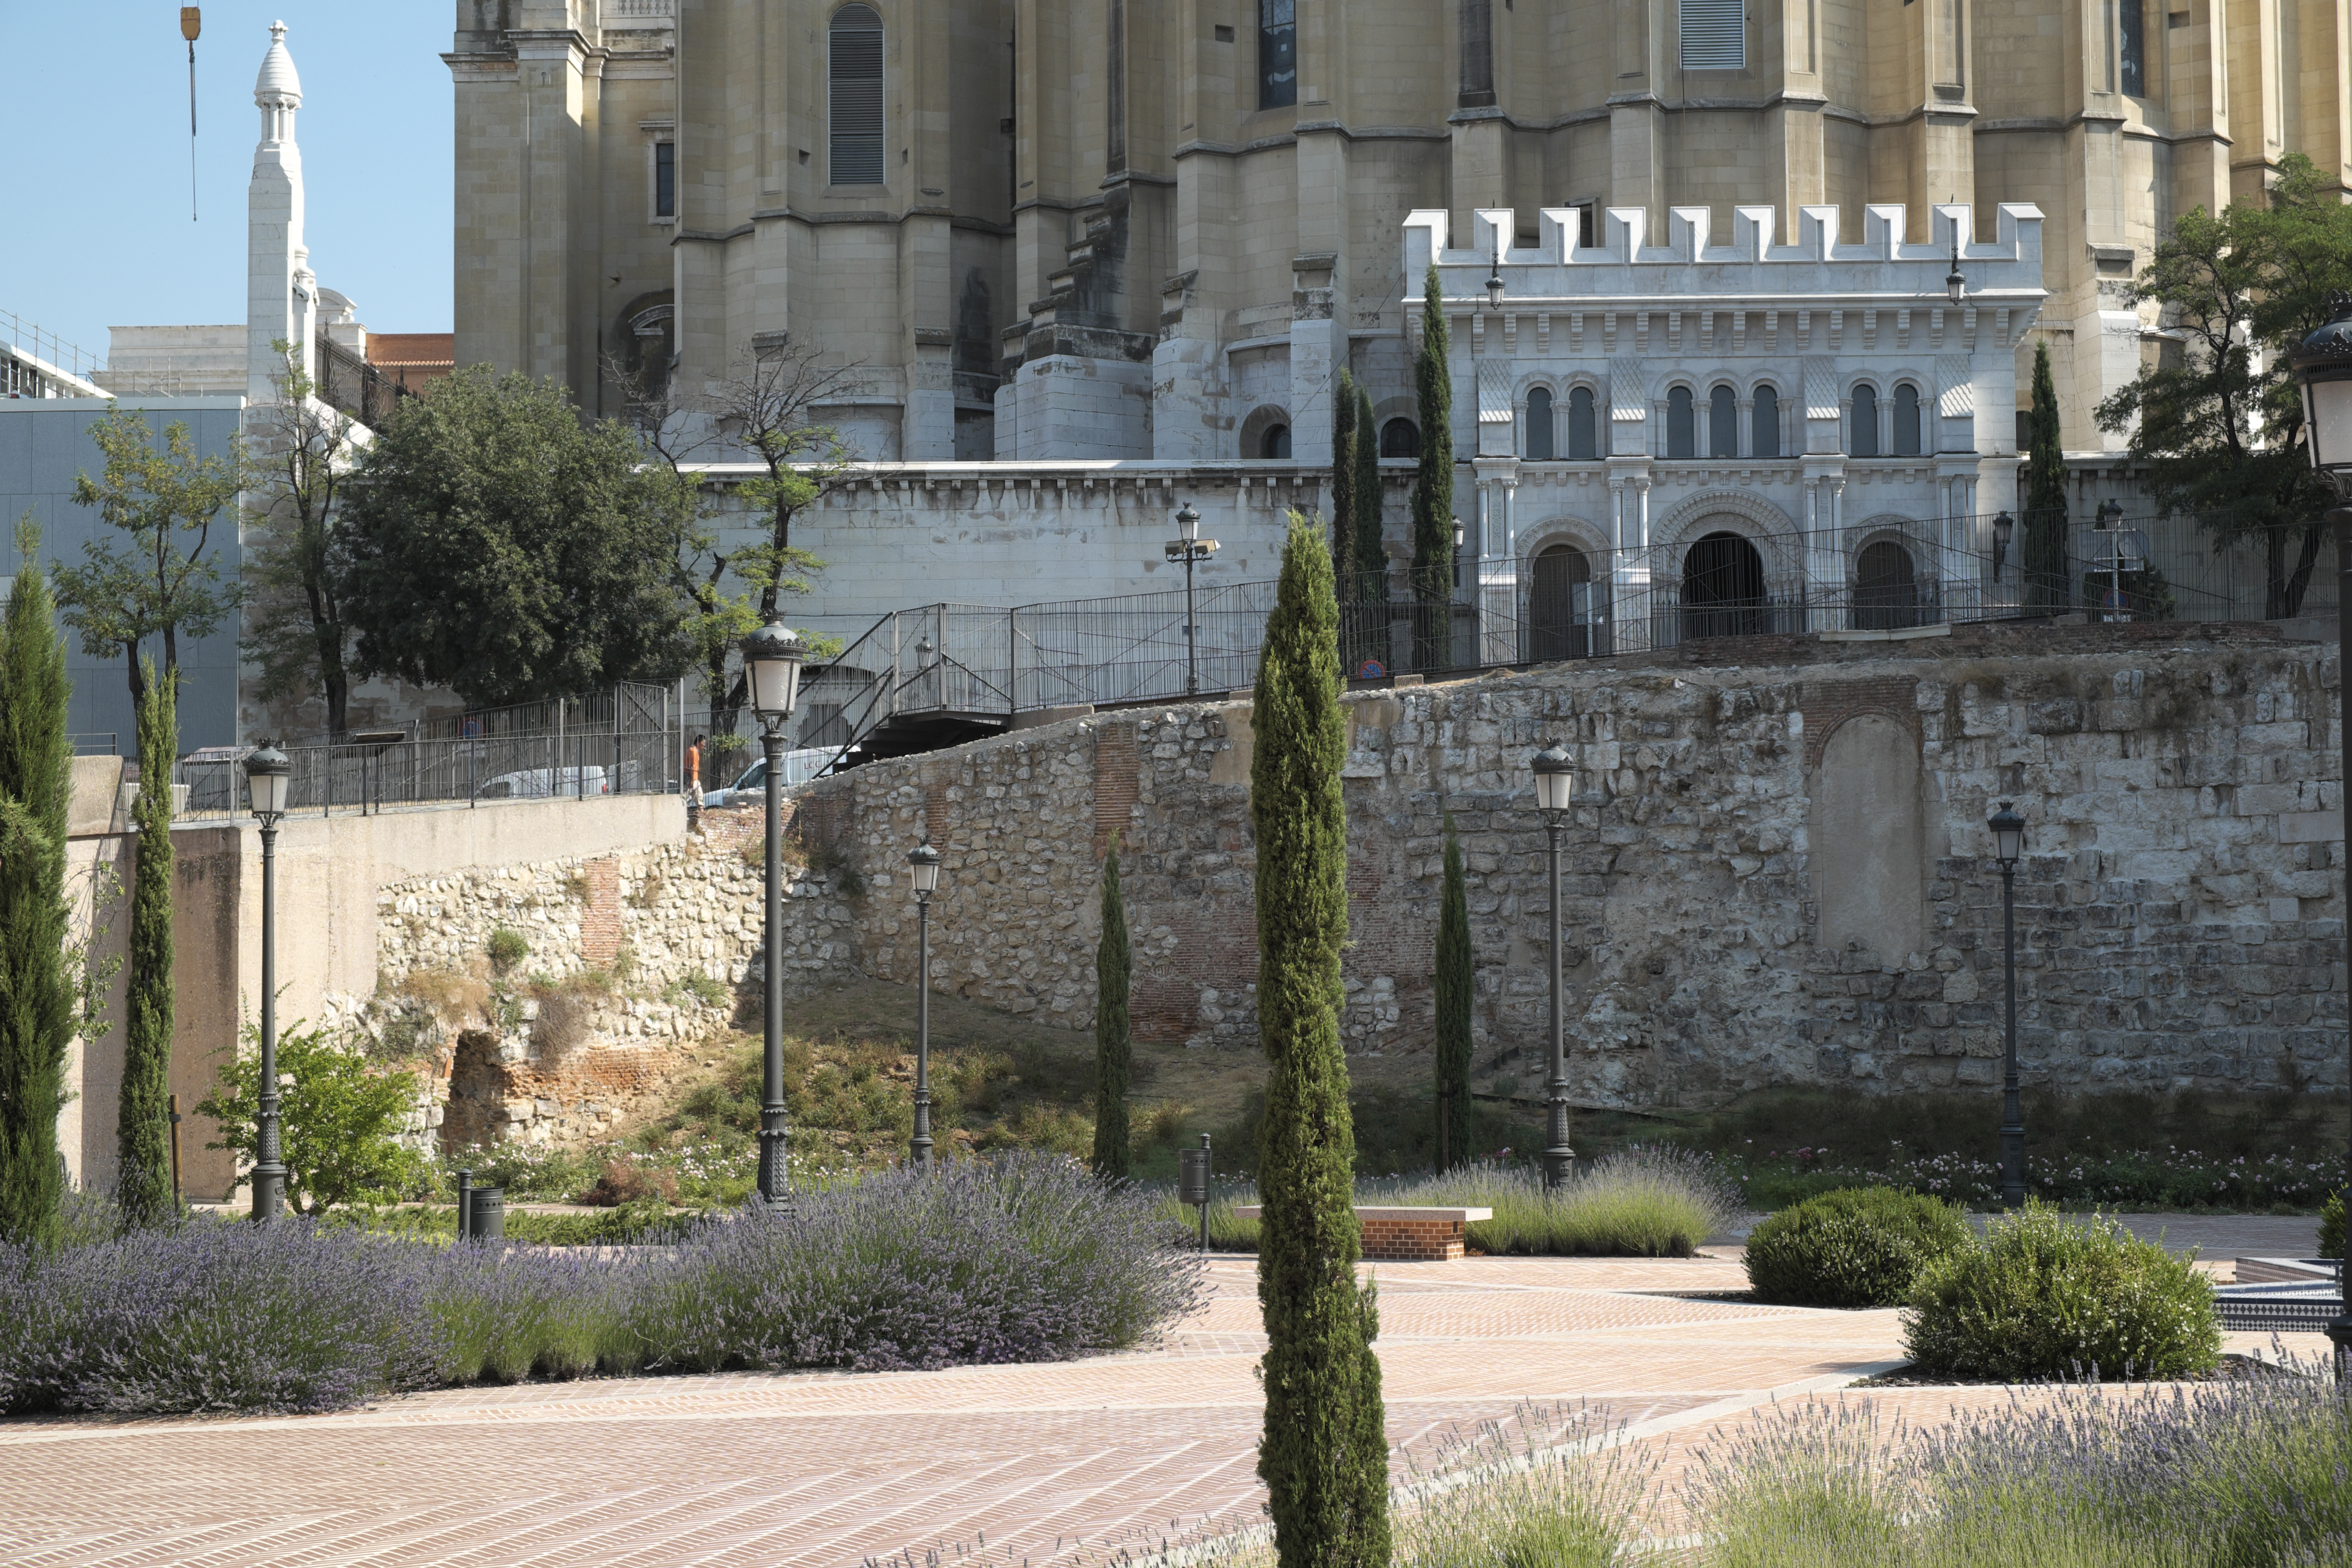
\includegraphics[scale=0.33]{img/Muralla.jpg}
\\
\small{Fuente: Wikipedia Commons.}
\end{figure}
\FloatBarrier


%%%%%%%%%%%%%%%%%%%%%%%%%%%%%%%%%%%%%%%%%%%%%%%%%%%%%%%%%%%%%%%%%%%%%%%%%%
%%%%%%%%%%%%%%%%%%%%%%%%%%%%%%%%%%%%%%%%%%%%%%%%%%%%%%%%%%%%%%%%%%%%%%%%%%
%%%%%%%%%%%%%%%%%%%%%%%%%%%%%%%%%%%%%%%%%%%%%%%%%%%%%%%%%%%%%%%%%%%%%%%%%%
%%%%%%%%%%%%%%%            TEMPORALIZACIÓN           %%%%%%%%%%%%%%%%%%%%%
%%%%%%%%%%%%%%%%%%%%%%%%%%%%%%%%%%%%%%%%%%%%%%%%%%%%%%%%%%%%%%%%%%%%%%%%%%
%%%%%%%%%%%%%%%%%%%%%%%%%%%%%%%%%%%%%%%%%%%%%%%%%%%%%%%%%%%%%%%%%%%%%%%%%%
%%%%%%%%%%%%%%%%%%%%%%%%%%%%%%%%%%%%%%%%%%%%%%%%%%%%%%%%%%%%%%%%%%%%%%%%%%
%%%%%%%%%%%%%%%%%%%%%%%%%%%%%%%%%%%%%%%%%%%%%%%%%%%%%%%%%%%%%%%%%%%%%%%%%%


\subsection{Temporalización}

La unidad didáctica se divide en 10 sesiones. 
%
Una explicación completamente desarrollada se encuentra en el apéndice \ref{app:todo}.


\label{ResumenSesion1}
%
La primera sesión es introductoria.
%
Se explicará la gamificación y su narrativa. 
%
Además, se crearán los grupos de trabajo para cuando sea necesario trabajar en equipo.
%
Hasta la finalización de la sesión se realizará un \textit{Kahoot} con el que repasar contenidos y conceptos que deberían saber de años anteriores.

\label{ResumenSesion2}
%
En la segunda sesión se trabajará la introducción a los polinomios, dentro de la narrativa de la gamificación. 
%
Los alumnos trabajaran autónomamente en un reto, cuya correcta resolución otorgará el logro \ref{logro::investigador_apto}.
%
En caso de que el trabajo en clase se haya desarrollado satisfactoriamente y todos los alumnos hayan conseguido descifrar el acertijo, se propondrá un pequeño test online (incluido en el anexo \ref{test:ses1}).
%
Excepcionalmente, en el caso de que el trabajo haya resultado muy complicado a los alumnos se podría emplear una sesión más en realizar los ejercicios del test en clase, con las explicaciones pertinentes del profesor.

\label{ResumenSesion3}
%
En la tercera sesión se procederá a una exposición por parte del profesor sobre la multiplicación de polinomios y los alumnos se enfrentarán a otro reto, esta vez por grupos debido al incremento de dificultad.
%
Para trabajar en casa se les propondrán varios ejercicios en la plataforma online de los que tendrán que seleccionar un número determinado. 
%
En principio serían 3, pero este valor puede ser modificado dependiendo del desempeño de los alumnos durante la sesión.
%
Cada ejercicio tendrá asociado una puntuación: los ejercicios más difíciles otorgan más puntos, los ejercicios más fáciles, menos puntos.

\label{ResumenSesion4}
%
La siguiente sesión se desarrollará con un esquema muy parecido, salvo que el contenido a trabajar será la división de polinomios.
%
Sin embargo, el trabajo en casa de esta sesión no será para practicar habilidades matemáticas sino para involucrarse más con la narrativa de la gamificación.

\label{ResumenSesion5}
%
En la quinta sesión se pondrá en marcha la posibilidad de conseguir un logro nuevo, \ref{logro::avizor}, por la identificación y resolución de una identidad notable.
%
La sesión transcurrirá con explicaciones por parte del profesor y ejemplos resueltos en la pizarra (en los que los alumnos podrán obtener subniveles del logro), seguidos de trabajo autónomo por parte del alumno.
%
No se propone trabajo para realizar extraescolarmente.

\label{ResumenSesion6}
%
La siguiente sesión se dividirá en 2 partes. 
%
Se explicará el algoritmo de Ruffini para dividir y se les propondrá el mismo desafío que en la sesión 3, el de las divisiones.
%
De esta manera podrán comprobar el potencial del algoritmo, ya que deberían emplear bastante menos tiempo en su resolución.
%
Una vez entendido y practicado Ruffini como algoritmo de división, se procederá a explicar cómo se puede factorizar un polinomio utilizando este algoritmo y se realizarán ejercicios prácticos.
%
Para trabajar en casa se propondrán ejercicios en \textit{edmodo} con el esquema utilizado anteriormente.
%
%En estos deberes se incorporará un vídeo con la explicación teórica sobre la factorización de polinomios con coeficiente principal distinto de 1.


\label{ResumenSesion7}
%
\label{ResumenSesion8}
%
En las siguientes 2 sesiones se propondrá un desafío complicado que implica aplicar con soltura todos los conocimientos aprendidos además de seguir aplicando conocimiento de años anteriores.
%
En la primera sesión se trabajará individualmente (cada miembro del equipo tendrá una ficha ligeramente diferente) y la segunda se trabajará colaborativamente.
%
Para la segunda sesión será necesario que los alumnos hayan finalizado con éxito sus partes individuales, ya que el equipo necesitará los resultados obtenidos en la parte individual.

\label{ResumenSesion9}
%
En la última sesión, no necesariamente la sesión siguiente, tendrá lugar el examen de la unidad.



\subsection{Recursos}

\subsubsection{Recopilación de los elementos de la gamificación }

Los recursos utilizados serán los propios desarrollados para esta Unidad Didáctica acompañadas del libro de referencia \cite{MareaVerde}.
%
Entre los recursos desarrollados se encuentran la utilización de la plataforma \textit{edmodo} para la resolución de ejercicios, los materiales didácticos disponibles en el aula para las exposiciones por parte del docente y la plataforma online \textit{Kahoot} para la sesión introductoria.

Por otro lado, se disponen de todos los recursos propios de esta gamificación.
%
Dichos recursos se encuentran descritos en las tablas \ref{Gamify:resumen} y \ref{tbl:tienda}.



\begin{longtable}{|m{0.06\linewidth}|m{0.28\linewidth}|m{0.52\linewidth}|}
\caption{Recopilación de los elementos de la gamificación utilizados}
\label{Gamify:resumen}\\
\hline
\textbf{ID} & \textbf{Nombre} & \textbf{Descripción}\\\hline
\endhead
EG1\labeltext{EG1}{puntos} & Puntos de reputación & Todos los puntos que se obtienen son de reputación.
%
El profesor podrá otorgar puntos de reputación a los alumnos por hacer preguntas interesantes o ayudarse entre ellos.
\\\hline
EG2\labeltext{EG2}{apto} & Logro \ref{logro::investigador_apto} & Se consigue por la resolución del \textit{Kahoot} realizado en la sesión introductoria.\\\hline
EG3\labeltext{EG3}{nato} & Logro \ref{logro::investigador_nato} & Se consigue mediante la correcta resolución del primer ejercicio autónomo propuesto en el aula.\\\hline
EG4\labeltext{EG4}{context} & Logro \ref{logro::contextualizador} & Este logro tiene niveles. Se obtendrá un nivel por la aplicación de alguno de los contenidos de la clase de matemáticas en su vida cotidiana y su posterior explicación a la clase.\\\hline
EG5\labeltext{EG5}{comp} & Logro \ref{logro::investigador_comprometido} & Se consigue un nivel del logro por la realización de los deberes mínimos el primer día y 2 niveles por la realización de todos los deberes del primer día.\\\hline
EG6\labeltext{EG6}{avizor} & Logro \ref{logro::avizor} & Este logro también tiene niveles y 3 subniveles por nivel. 
%
Se obtendrá un subnivel del logro cada vez que se identifique y se resuelva con éxito una identidad notable durante una actividad conjunta de toda la clase (como puede ser durante una exposición del docente).\\\hline
EG7\labeltext{EG7}{narrativa} & Narrativa & Los alumnos son investigadores de unos manuscritos árabes sobre Matemáticas y tienen que desenterrar un tesoro escondido en Madrid.\\\hline
EG8\labeltext{EG8}{explorador} & Medalla \logro{Explorador}{explorador} & Obtenible al realizarse un \textit{selfy} en el lugar del tesoro.\\\hline
EG9\labeltext{EG9}{eleccion} & Elección & Posibilidad de elección de los deberes a realizar (Mecánica de la gamificación). \\\hline
EG10\labeltext{EG10}{feedback} & Retroalimentación inmediata & Utilización de una herramienta online para aportar retroalimentación inmediata a los alumnos al realizar los deberes \\\hline
EG11\labeltext{EG11}{fichas} & Economía de fichas & Los puntos de reputación sirven como moneda en una economía. Los puntos invertidos en compras se pierden.
%
En la tienda se pueden comprar ciertos privilegios descritos en \ref{tbl:tienda}. \\\hline
\end{longtable}

\begin{table}[hptb]
\centering
\caption{Artículos de la economía de fichas}
\label{tbl:tienda}
\begin{tabular}{|m{0.15\linewidth}|m{0.18\linewidth}|m{0.53\linewidth}|}
\hline
\textbf{Puntos} & \textbf{Nombre} & \textbf{Descripción} \\ \hline
$200$ & ExtraQuizz	& Aumentar en 1 el número de ejercicios que se pueden hacer en \textit{edmodo} para ganar puntos.\\\hline
$(x^2-x+1)·320$ & TeacherQuizz & $x$ preguntas directas (de sí o no) y precisas\footnotemark al docente en el examen\\\hline
$400$ & Miniatura algebraica & Una botella de Klein impresa en 3D \citep{Klein} \\\hline
$200$ & Bonus x2 & Obtención de un bonus duplicador de puntos para una sesión.\\\hline
%$r$ &  &  \\\hline
\end{tabular}
\footnotetext{Preguntas del tipo: ¿Este ejercicio está bien? es demasiado ambigua y no sería válida. Preguntas como: ¿Con el ejercicio así obtendría la máxima puntuación? sí sería válida.
%
El grado de precisión de una pregunta será competencia única del docente en el momento del examen.}
\end{table}

\FloatBarrier

\subsection{Evaluación}

\label{eval}
%
La evaluación que se propone para esta unidad didáctica es a través de un examen incluido en el anexo \ref{app:examen} con la ponderación que estuviera establecida en la \gls{PDA} y el trabajo de clase, que se medirá mediante los puntos y medallas obtenidos por cada alumno.

Para establecer ponderación de las medallas y de los puntos de reputación para obtener la calificación del trabajo de clase se propone el siguiente sistema:
%
de los 10 puntos de actitud y trabajo en clase, hasta un máximo de 6 puntos se podrán obtener mediante logros, otorgando cada logro un punto\footnote{2 niveles de un mismo logro otorgarán 2 puntos} y hasta un máximo de 4 puntos se podrán obtener mediante puntos de reputación, mediante una regla de 3, correspondiendo 4 puntos de la calificación con 800 puntos de reputación\footnote{El máximo número de puntos de reputación que se pueden obtener sin bonus de ningún tipo ni por premios otorgados por el docente son 1160.} y 0 puntos en la calificación con 0 puntos de reputación.


La evaluación a través de un examen tiene varias ventajas:
%
la primera es la facilidad de la incorporación de esta unidad didáctica en un curso que ya funcione con otras metodologías.
%
No hace falta modificar los criterios de evaluación que se hubieran establecido para evaluar a los alumnos.

Además, permite y facilita la experimentación.
%
Se pueden comparar los resultados del aprendizaje mediante un examen en un curso que ha participado en la gamificación frente a un curso que haya recibido las sesiones mediante otras metodologías.
%
En el caso de que esta estrategia metodológica fuese adoptada por un único docente en un departamento, la posible experimentación permitiría iniciar un diálogo y debate sobre la incorporación de la gamificación por parte de otros docentes, incluso en otros cursos.

Dicho lo cual, sería injusto no comentar que la evaluación mediante un examen no es la mejor manera de realizar una evaluación justa que asegure la adquisición de las competencias y el aprendizaje duradero los contenidos.
%
Se podrían utilizar rúbricas, por ejemplo, que permitirían una evaluación mucho más exhaustiva y personalizada.
%
Sin embargo, se ha preferido optar por el examen por todo lo expuesto anteriormente.



%%%%%%%%%%%%%%%%%%%%%%%%%%%%%%%%%%%%%%%%%%%%%%%%%%%%%%%%%%%%%%%%%%%%%%%%
%%%%%%%%%%%%%%%%%%%%%%%%%%%%%%%%%%%%%%%%%%%%%%%%%%%%%%%%%%%%%%%%%%%%%%%%
%%%%%%%%%%%%%%%%%%%%%%%%%%%%%%%%%%%%%%%%%%%%%%%%%%%%%%%%%%%%%%%%%%%%%%%%
%%%%%%%%%%%%%%%%%%%%%%%%%%%%%%%%%%%%%%%%%%%%%%%%%%%%%%%%%%%%%%%%%%%%%%%%
%%%%%%%%%%%%%%%%%%%%%%%%%%%%%%%%%%%%%%%%%%%%%%%%%%%%%%%%%%%%%%%%%%%%%%%%
%%%%%%%%%%%%%%%%%%%%%%%%%%%%%%%%%%%%%%%%%%%%%%%%%%%%%%%%%%%%%%%%%%%%%%%%
%%%%%%%%%%%%%%%%%%%%%%%%%%%%%%%%%%%%%%%%%%%%%%%%%%%%%%%%%%%%%%%%%%%%%%%%
%%%%%%%%%%%%%%%%%%%%%%%%%%%%%%%%%%%%%%%%%%%%%%%%%%%%%%%%%%%%%%%%%%%%%%%%
%%%%%%%%%%%%%%%%%%%%%%%%%%%%%%%%%%%%%%%%%%%%%%%%%%%%%%%%%%%%%%%%%%%%%%%%
%%%%%%%%%%%%%%%%%%%%%%%%%%%%%%%%%%%%%%%%%%%%%%%%%%%%%%%%%%%%%%%%%%%%%%%%
%%%%%%%%%%%%%%%%%%%%%%%%%%%%%%%%%%%%%%%%%%%%%%%%%%%%%%%%%%%%%%%%%%%%%%%%
%%%%%%%%%%%%%%%%%%%%%%%%%%%%%%%%%%%%%%%%%%%%%%%%%%%%%%%%%%%%%%%%%%%%%%%%
%%%%%%%%%%%%%%%%%%%%%%%%%%%%%%%%%%%%%%%%%%%%%%%%%%%%%%%%%%%%%%%%%%%%%%%%
%%%%%%%%%%%%%%%%%%%%%%%%%%%%%%%%%%%%%%%%%%%%%%%%%%%%%%%%%%%%%%%%%%%%%%%%
%%%%%%%%%%%%%%%%%%%%%%%%%%%%%%%%%%%%%%%%%%%%%%%%%%%%%%%%%%%%%%%%%%%%%%%%
%%%%%%%%%%%%%%%%%%%%%%%%%%%%%%%%%%%%%%%%%%%%%%%%%%%%%%%%%%%%%%%%%%%%%%%%
%%%%%%%%%%%%%%%%%%%%%%%%%%%%%%%%%%%%%%%%%%%%%%%%%%%%%%%%%%%%%%%%%%%%%%%%
%%%%%%%%%%%%%%%%%%%%%%%%%%%%%%%%%%%%%%%%%%%%%%%%%%%%%%%%%%%%%%%%%%%%%%%%
%%%%%%%%%%%%%%%%%%%%%%%%%%%%%%%%%%%%%%%%%%%%%%%%%%%%%%%%%%%%%%%%%%%%%%%%
%%%%%%%%%%%%%%%%%%%%%%%%%%%%%%%%%%%%%%%%%%%%%%%%%%%%%%%%%%%%%%%%%%%%%%%%
%%%%%%%%%%%%%%%%%%%%%%%%%%%%%%%%%%%%%%%%%%%%%%%%%%%%%%%%%%%%%%%%%%%%%%%%
%%%%%%%%%%%%%%%%%%%%%%%%%%%%%%%%%%%%%%%%%%%%%%%%%%%%%%%%%%%%%%%%%%%%%%%%
%%%%%%%%%%%%%%%%%%%%%%%%%%%%%%%%%%%%%%%%%%%%%%%%%%%%%%%%%%%%%%%%%%%%%%%%
%%%%%%%%%%%%%%%%%%%%%%%%%%%%%%%%%%%%%%%%%%%%%%%%%%%%%%%%%%%%%%%%%%%%%%%%
%%%%%%%%%%%%%%%%%%%%%%%%%%%%%%%%%%%%%%%%%%%%%%%%%%%%%%%%%%%%%%%%%%%%%%%%
%%%%%%%%%%%%%%%%%%%%%%%%%%%%%%%%%%%%%%%%%%%%%%%%%%%%%%%%%%%%%%%%%%%%%%%%
%%%%%%%%%%%%%%%%%%%%%%%%%%%%%%%%%%%%%%%%%%%%%%%%%%%%%%%%%%%%%%%%%%%%%%%%



\section{Evaluación de la gamificación}

%Anteriormente\crossref{ (ver \ref{eval})} se ha esbozado una posible experimentación para evaluar la gamificación que ahora va a ser desarrollada.

Para evaluar una metodología se pueden diferentes varios aspectos.
%
En esta propuesta nos centramos en 2 aspectos concretos:
%
cómo funciona la gamificación frente a otras metodologías y cómo mejorar la  gamificación realizada.

\label{evalGami}

\subsection{La Gamificación frente a otras metodologías}

Para valorar si esta propuesta metodológica mejora otras propuestas metodológicas se puede llevar a cabo el siguiente experimento.

Se elige aleatoriamente la mitad truncada de los grupos de Matemáticas orientadas a las Ciencias Académicas de 3º de la ESO.
%
Estos grupos formarán el grupo experimental y los grupos no seleccionados formarán el grupo control.

Tanto para el grupo experimental como para el grupo control se especificará una fecha en la que tener el examen de la unidad.
%
Todos los alumnos de todos los grupos, si es posible, realizarán el examen a la vez.
%
Se tomarán las medidas necesarias para que todos los grupos tengan el mismo número de sesiones, ya que podría ocurrir que un grupo perdiera sesiones de Matemáticas por días festivos.
%
Estas medidas eliminan algunas amenazas a la validez del experimento.

Una vez fijados estos parámetros iniciales, se comenzará la Unidad Didáctica la misma semana en todos los grupos.
%
En el grupo experimental se utilizará esta propuesta metodológica mientras que en el grupo control se utilizará la metodología establecida por defecto en el centro.

Al final de las sesiones se dispone de un instrumento de medida igual para todos los participantes: el examen de la unidad.
%
De esta manera se puede comparar la gamificación con la metodología empleada en el grupo control.
%
Se procederá a realizar un contraste estadístico para determinar el grado de diferencia entre la distribución de las notas obtenidas en el grupo experimental frente a las notas obtenidas en el grupo control.


\subsection{Autoevaluación}

Por otro lado, es fundamental saber si la gamificación tal como se ha llevado a cabo ha merecido la pena, qué aspectos son mejorables y cuáles hay que mantener.
%
Debido a las dificultades que se encuentran al querer plantear una experimentación utilizando esta unidad didáctica concreta se propone que el docente realice un informe cualitativo a medida que van avanzando las sesiones y que al final se realice una autoevaluación buscando mejorar la propuesta.

En esta autoevaluación se debe valorar el grado de ajuste de la dificultad de los ejercicios propuestos a las habilidades de los alumnos, 
%
cómo han funcionado trabajando en grupo frente a trabajar individualmente, cómo ha funcionado la realización de los deberes online, etc.

